\chapter{Enantiomorphing Chiral Nanostructures}\label{sec:results:EnantiomorphingChiralCrosses}


Sections of this chapter have been copied verbatim from the (published) manuscript \textit{``Enantiomorphing Chiral Plasmonic Nanostructures: A Counterintuitive Sign Reversal of the Nonlinear Circular Dichroism''}, Joel T. Collins et. al. \cite{Collins2018}. 
Experiments were planned by V. K. Valev. Samples were prepared by N. V. S. Braz and P. A. Warburton. SHG microscopy experiments were executed by V. K. Valev, E. Slenders and M. Ameloot. Linear scattering spectra were obtained by myself and C. Kuppe, and analysed by myself. Near-field and scattering simulations were performed by X. Zheng and G. A. E. Vandenbosch. Numerical simulations of the linear far-field reflection CID were performed by S. Zu and Z. Fang. 
Analysis of the nonlinear microscopy data was performed by myself, with Python code including sections written by V. K. Valev. The formulation and analysis of modal circular-dichroism based on the near-field simulations was also performed by myself. I produced the manuscript draft, and all authors have subsiquently contributed. 

\bigskip \noindent
Plasmonic nanostructures have demonstrated a remarkable ability to control light in ways never observed in nature, as the optical response is closely linked to their flexible geometric design.
Due to lack of mirror symmetry, chiral nanostructures allow twisted electric field ``hotspots'' to form at the material surface. 
These hotspots depend strongly on the optical wavelength and nanostructure geometry.
Understanding the properties of these chiral hotspots is crucial for their applications; for instance, in enhancing the optical interactions with chiral molecules. 
Here, the results of an elegant experiment are presented: by designing 35 intermediate geometries, the structure is ``enantiomorphed'' from one handedness to the other, passing through an achiral geometry. 
Nonlinear multiphoton microscopy is used to demonstrate a new kind of double-bisignate circular dichroism due to enantiomorphing, rather than wavelength change.
From group theory, a fundamental origin of this plasmonic chiroptical response is proposed. The analysis allows the optimization of plasmonic chiroptical materials.

\section{Introduction}\label{sec:results:EnantiomorphingChiralCrosses:introduction}
Throughout the 19th and most of the 20th century, chirality has been primarily associated with chemistry. However, whereas chirality can be crucial for understanding molecules, molecules are not best suited for understanding chirality.  
Ideally, we would like to be able to vary the chirality of a particular structure, i.e., to follow chirality parameter values as chiral systems transition from one form into another. However, it is not possible to freely control the geometric properties of molecules. Modern nanofabrication techniques have lifted this limitation on tuning chiral parameters.

Using modern nanofabrication, it is possible to explore the evolution of chiral forms, by preparing numerous intermediate geometries. This is important because it opens the possibility to tune and optimize the chirality parameters, which enable interesting properties. For instance, by maximizing the geometric chirality parameter, it is possible to achieve negative refractive index materials \cite{Pendry2004a}. Such materials could lead to super-lenses \cite{Khorasaninejad2016}, and various applications that depend on the control of circularly polarized light (CPL). In turn, CPL could find applications in spintronics \cite{Farshchi2011b} and quantum computing \cite{Wagenknecht2010a, Sherson2006a}.
Moreover, by optimizing \textit{optical chirality} (section~\ref{sec:background:Chirality:opticalchirality}) it has been shown that ``superchiral'' light configurations can be achieved. Importantly, optical chirality is particularly enhanced at the surface of chiral plasmonic nanostructures (section~\ref{sec:background:Plasmonics:superchiral}), resulting in large enhancements in measurable circular dichroism (CD).

Despite the advantages of creating intermediate geometries, it is rare to find studies where these have been investigated in detail. Between two enantiomorphs, there can be several path- ways for intermediate geometries and those might be quite different (Figure~\ref{fig:results:EnantiomorphingChiralCrosses:setup}a). 
Also, a priory, it is not clear what the best number of intermediate geometries should be. Indeed this is highly dependent on the geometric and material properties of the structures, as well as on the wavelength ranges used. In the literature, examples can be found of studying both enantio- morphs of a structure, its achiral variant, and a small number of intermediate steps only \cite{Zu2016}. Consequently, important and interesting behaviour can go unnoticed.

\begin{figure}[htb]	
    \centering	
    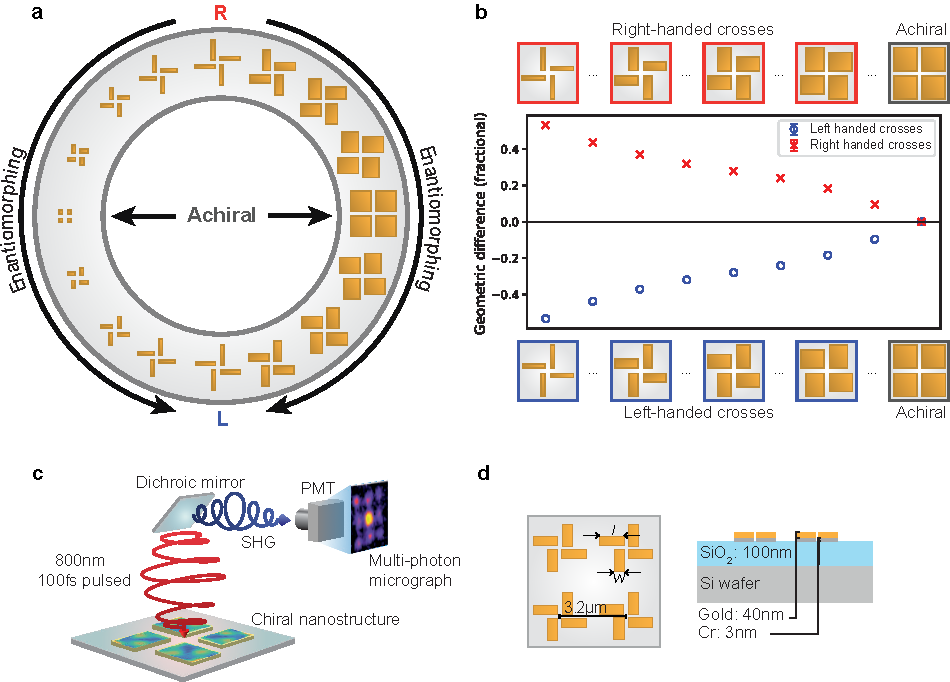
\includegraphics[scale=1]{./figures/results/EnantiomorphingChiralCrosses/setup.pdf}
    \caption{\label{fig:results:EnantiomorphingChiralCrosses:setup}
    \textbf{a)} Representation of two possible pathways to enantiomorph a right-handed structure (R) into a left-handed structure (L), through an achiral geometry. Here, we examine the pathway on the right side of the circle. \textbf{b)} As the left-handed chiral crosses change into achiral square structures and into right-handed chiral crosses, the chiral geometric difference diminishes until it reaches 0 in the achiral case and then reverse its value. \textbf{c)} Schematic diagram of the multiphoton microscopy experiments. \textbf{d)} Geometry and depth profile of the chiral crosses samples.}	
\end{figure}

Here, we developed an experiment impossible to perform with chiral molecules: by designing 35 intermediate geometries, we ``enantiomorph'' plasmonic nanostructures from one handedness to the other, passing through an achiral geometry. 
We demonstrate a bisignate circular intensity difference (CID) due to enantiomorphing, rather than wavelength change, in the nonlinear emission from near-field hotspots. Contrary to what would be expected from pure geometric considerations, the nonlinear chiroptical signal reverses sign thrice, i.e., it is double-bisignate. In order to understand this result, we perform a full modal analysis of the structures in combination with group theory. 
We find that, regardless of their handedness, chiral nanostructures contain modes that can be excited by both left and right circularly polarized (LCP and RCP) light. Furthermore, which modes are dominant (i.e., couple strongest to light) depends on the wavelength or the shape/dimensions of the nanostructure. It is therefore perfectly possible to engineer chiral nano- materials that, at a given wavelength, can only be excited with the ``wrong'' kind of CPL. 
Our findings offer the possibility of tuning chiroptical response by selecting particular electromagnetic modes, or sets of modes, among hundreds available, which can enable much more sensitive chiroptical control than what is currently available.

\section{Results}\label{sec:results:EnantiomorphingChiralCrosses:results}

We begin by presenting the purely geometric considerations. Starting with left-handed crosses, we morph their geometry in discrete steps, first into achiral squares and then into right-handed chiral crosses (Figure~\ref{fig:results:EnantiomorphingChiralCrosses:setup}b). For the purposes of comparison, we use a measure of ``chiral geometric difference'' (not to be confused with the geometric chirality parameter). 
This quantity describes the area of maximal overlap that can be achieved between left- and right-handed structures, by rotating and translating the two mirror-image shapes, relative to each other (Appendix~\ref{sec:appendix:ChiralGeoDiff}). 
As Figure~\ref{fig:results:EnantiomorphingChiralCrosses:setup}b shows, the chiral geometric difference diminishes until it reaches 0, in the achiral case. However, the chiroptical properties of nanostructures depend on more than geometry alone; without considering material effects, and the properties of the incident light, no direct connection can be made between chiral geometric difference and chiroptical effects. This measure of chirality is in stark contrast to the double-bisignate response found in our nonlinear CID measurements.

For our experiments, we made use of multiphoton microscopy performed with CPL illumination at 800 nm and schematized in Figure~\ref{fig:results:EnantiomorphingChiralCrosses:setup}c. The instrument was a standard commercial model. The collected light consisted mostly of the second harmonic generation (SHG). Specifically, a bandpass filter allowing $\SI{390}{\nano\m}$ to $\SI{465}{\nano\m}$ light was used and, although this filter passes a small part of two-photon luminescence signal, the SHG signal is clearly dominant in this spectral range. Since these nonlinear optical processes are enhanced in the regions of strong local field, \cite{Wang2013, Chen1983} they act as a sensitive far-field probe for local field effects. 

The samples are chiral crosses made of Au, deposited by electron beam lithography (EBL) on a Si substrate with a thermal oxide layer, and whose dimensions and depth profile are given in Figure~\ref{fig:results:EnantiomorphingChiralCrosses:setup}d. Each cross is composed of four separate nanostripes, with varying width $w$ and length $l$. The separation distance between nanostripes, at the centre of the crosses, is constant at $\SI{200}{\nano\m}$. The crosses are arranged in a $\SI{40}{\micro\m} \times \SI{40}{\micro\m}$ square array, with the distance between cross centres also kept constant at $\SI{3.2}{\micro\m}$. 

\begin{figure}[htb!]	
    \centering	
    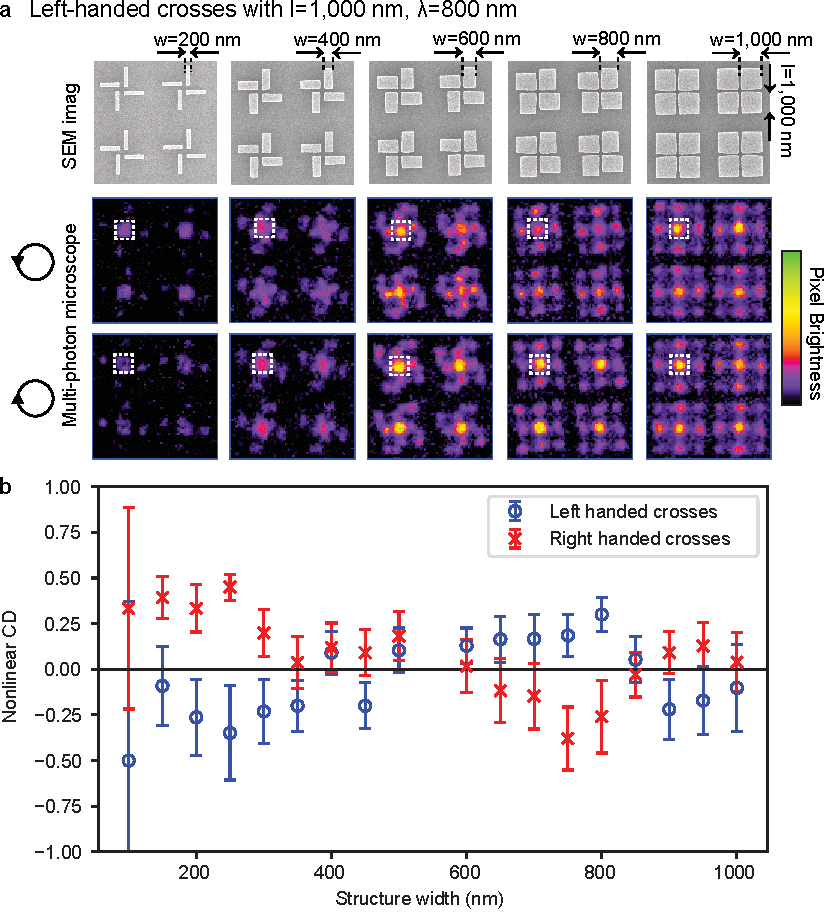
\includegraphics[scale=1]{./figures/results/EnantiomorphingChiralCrosses/l1000data.pdf}
    \caption{\label{fig:results:EnantiomorphingChiralCrosses:l1000data}
    Varying arm width of the nanostructure features at fixed l=1000nm. SEM images of 4 structure cells for each geometry \textbf{(a top)}, and SHG microscopy images \textbf{(a, lower)} under illumination from left and right circularly polarized light, at $\SI{800}{\nano\m}$ wavelength. Scale (right) corresponds to image pixel brightness. \textbf{b)} Measured total nonlinear CID under $\SI{800}{\nano\m}$ wavelength light is then calculated for each geometry. Our experiments reveal a counter-intuitive behavior for the second-harmonic generation circular dichroism (SHG-CID) – both the 0 value and the reversal occur before reaching the achiral geometry.}	
\end{figure}

Figure~\ref{fig:results:EnantiomorphingChiralCrosses:l1000data}a shows scanning electron microscopy (SEM) images of sample arrays. In these arrays, the length of the nanostripes is fixed ($\SI{1000}{\nano\m}$) and the width changes from $\SI{200}{\nano\m}$ to $\SI{1000}{\nano\m}$ in steps of $\SI{200}{\nano\m}$. Underneath each SEM are two corresponding multi-photon micrographs, obtained with LCP and RCP. The multi-photon microscopy images are color-coded for intensity and they show bright hotspots at the center of the chiral crosses (indicated with dashed-line squares for clarity). 
Similar hotspots have previously been observed at the center of G-shaped \cite{Valev2009a} and S-shaped \cite{Valev2014} nanostructured arrays. 
The hotspots correspond to a chiral coupling at the center of the unit cells that depends on the chirality of the nanostructures and the direction of CPL \cite{ Valev2014, Petralli-Mallow1993, Byers1994}. This dependence is expressed as a directly observable nonlinear circular intensity difference (CID). Interestingly though, in this set of samples, the nonlinear CID changes sign between the chiral crosses with nanostripe width  $\SI{200}{\nano\m}$ and $\SI{600}{\nano\m}$, even though the structures have the same handedness.

The nonlinear CID reversal can be seen more quantitatively in Figure~\ref{fig:results:EnantiomorphingChiralCrosses:l1000data}b. Here, the nonlinear CID is obtained from the detected light upon LCP or RCP illumination according to 
$(I_{RCP}^{MP}-I_{LCP}^{MP})/(I_{RCP}^{MP}+I_{LCP}^{MP})$. The individual multi-photon intensity terms $I_{RCP}^{MP}$ and $I_{LCP}^{MP}$ were obtained from the pixel intensity at the center of the chiral crosses, where the chiral coupling is maximum and the characteristic response is most pronounced. 
The nonlinear microscopy images obtained contain roughly 60 crosses of each type (normal and mirror), with separate images for LCP and RCP illumination. A Python script was used to specify the central regions of 25 crosses, with clearly damaged structured avoided. For each cross, a 5-pixel by 5-pixel square at the defined central region was intensity-averaged (pixel array at $\SI{0.09}{\micro\m}$ per pixel). This result was itself then averaged over 25 crosses to obtain a final intensity and statistical uncertainty for a particular orientation of cross (normal or mirror) and input polarization (LCP or RCP). This was done for each of the considered geometries. 
It should be noted that the SEM pictures in Figure~\ref{fig:results:EnantiomorphingChiralCrosses:l1000data}a are only a subset of the entire range of samples we studied. The full set started from $w= \SI{100}{\nano\m}$ and progressed to $w=\SI{1000}{\nano\m}$, in steps of $\SI{50}{\nano\m}$. 
Upon considering the nonlinear CID from all these samples, it is obvious that between $w=\SI{200}{\nano\m}$ and $w=\SI{800}{\nano\m}$, the chiroptical response is unambiguously reversed, i.e. with clearly separated error bars. The nonlinear CID that we measured is collected in the far-field and it is very different from the linear circular dichroism in the far-field. 

In the far-field, the linear CID response is demonstrated by FDTD simulations data that are displayed in Figure~\ref{fig:results:EnantiomorphingChiralCrosses:reflectionsim}. Additional linear scattering spectra simulations and experimental data are given in Appendix~\ref{sec:appendix:CrossesScatteringSpectra}. Clearly, the data in Figure~\ref{fig:results:EnantiomorphingChiralCrosses:reflectionsim} do not match those in Figure~\ref{fig:results:EnantiomorphingChiralCrosses:l1000data}b. One reason for this difference is that the nonlinear CID originates in the near-field, which is very different from the far-field in this kind of structures. To understand the observed reversal of the nonlinear CID, we need to examine the electromagnetic behaviour at the surface of the nanostructures. 

\begin{figure}[htb!]	
    \centering	
    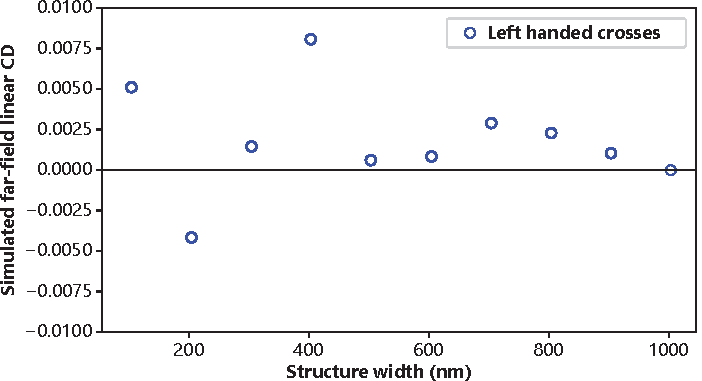
\includegraphics[scale=1]{./figures/results/EnantiomorphingChiralCrosses/reflection_sim.pdf}
    \caption{\label{fig:results:EnantiomorphingChiralCrosses:reflectionsim}
    Numerically-obtained far-field linear reflection CD for left-handed chiral cross structures. The lineshape of the linear CD response is significantly different to that obtained from nonlinear CID measurements.}	
\end{figure}

\section{Discussion}\label{sec:results:EnantiomorphingChiralCrosses:discussion}

\begin{figure}[htb!]	
    \centering	
    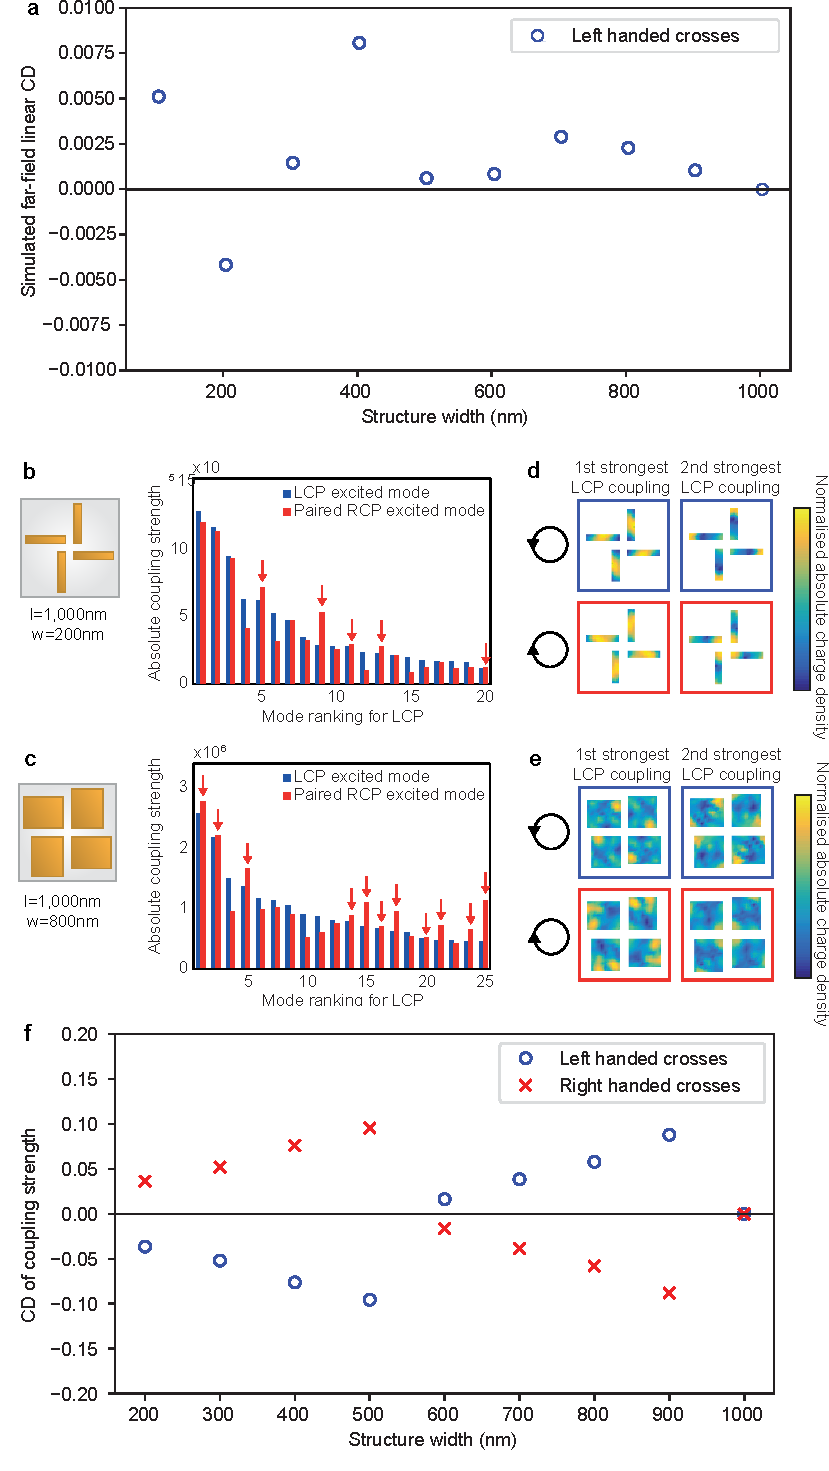
\includegraphics[scale=1]{./figures/results/EnantiomorphingChiralCrosses/l1000modes.pdf}
    \caption{\label{fig:results:EnantiomorphingChiralCrosses:l1000modes}
    \textbf{a-e}. Simulation results showing modal composition of chiroptical response. Modal analysis of structures with arm length 1000nm, width 200nm \textbf{(a)} and 800nm \textbf{(b)}. The most LCP-dominant modes for each structure are plotted showing both LCP coupling strength (blue) and the correlated-mode RCP coupling strength (red). Modes coupling stronger to RCP than LCP are marked with arrows. Examples of individual modes (normalized absolute charge density) are shown for width $\SI{200}{\nano\m}$ \textbf{(c)} and 800nm \textbf{(d)}. The total coupling strength CID as defined in equation~\ref{eq:background:ChiropticalEffects:couplingCD} is plotted for varying arm width, at fixed $l=\SI{1000}{\nano\m}$ under $\SI{800}{\nano\m}$ wavelength light \textbf{(e)}.}	
\end{figure}

For each nanostructure examined, the induced current (and charge) flowing in the structure due to an incident field was obtained by X. Zheng and G. A. E. Vandenbosch using the methods detailed in references \cite{Collins2018, Zheng2012}. For a given structure, the full induced current solution $\mathbf{J}$ is characterized by a set of modes $\mathbf{J_n}$ and corresponding eigenvalues $\lambda_{n}$. Each structure is associated with a different set of modes, and the amplitudes of each mode describe their coupling strengths to a particular incident field.
These methods are well established, but here the analysis was taken further by making use of group theory. Each available mode associated with a given structure geometry can be placed in one of four orthogonal irreducible representations $\Gamma _{j = 1,2,3,4}$. These representations correspond to exclusive excitation with either the two orthogonal linear polarizations ($\Gamma _{1}$ for horizontal and $\Gamma _{2}$ for vertical) or the two circular polarizations ($\Gamma _{3}$ for LCP and $\Gamma _{4}$ for RCP). 
Importantly, each mode in the 3rd irreducible representation has a “correlated” mode in the 4th irreducible representation, with identical eigenvalues forming an ``accidentally degenerate pair''. 
Crucially, the LCP coupling coefficient of a given $\Gamma _{3}$ mode may be different from the RCP coupling coefficient of the correlated $\Gamma _{4}$ mode. 
This difference in a mode pair's ability to couple to LCP and RCP incident light can be seen as a type of modal CID, and is shown in Figure~\ref{fig:results:EnantiomorphingChiralCrosses:l1000modes}b, c. 

Figure~\ref{fig:results:EnantiomorphingChiralCrosses:l1000modes}b shows pairs of correlated modes in the structures with width $\SI{200}{\nano\m}$. In blue, the $\Gamma _{3}$ modes are ranked according to their coupling coefficient to LCP. The correlated $\Gamma _{4}$ modes are shown in red, please note these only couple to RCP. In an achiral structure, both the blue and red sets would have identical values and ranking. Not surprisingly, the presence of chirality in the structure breaks the symmetry and, overall, the blue modes have higher coupling coefficients. 
But counter-intuitively, we also find that, in some pairs, the red modes have higher coupling coefficients. This means that, for such modes, light of the ``wrong chirality'' couples more efficiently to the chirality of the nanostructure. An example of this behaviour is indicated with an arrow on the figure. As we will see next, the exception can become the rule as we continue changing the cross width towards an achiral structure.

Figure~\ref{fig:results:EnantiomorphingChiralCrosses:l1000modes}c shows pairs of correlated modes in the structures with width $\SI{800}{\nano\m}$. Here, there are more red-dominant pairs of correlated modes than in Figure~\ref{fig:results:EnantiomorphingChiralCrosses:l1000modes}b, to the point that the overall calculated near-field CID is reversed, as in the experimental observation. Therefore, in these plasmonic nanostructures, the chiroptical response originates from the superposition of all the individual modal responses. 
The modes themselves represent complex spatial distributions of the charge density; as an illustration, the first and second modes from Figure~\ref{fig:results:EnantiomorphingChiralCrosses:l1000modes}b and \ref{fig:results:EnantiomorphingChiralCrosses:l1000modes}c are shown in Figure~\ref{fig:results:EnantiomorphingChiralCrosses:l1000modes}d and \ref{fig:results:EnantiomorphingChiralCrosses:l1000modes}e, respectively.
Since the near-field intensity is directly related to the total charge density, regions of high charge density will result in SHG hotspots (via local fields) on the structure surface. Therefore, differences in the coupling of charge density modes to LCP and RCP light are directly responsible for the observed SHG-CID.

Mathematically, the overall near-field CID originates from the full solution $\mathbf{J}$ obtained by linearly superposing the contributions from all eigenmodes $\mathbf{J_n}$, 

\begin{equation}\label{eq:background:ChiropticalEffects:totalSolution}	
	\mathbf{J} (\mathbf{r}, \omega) = \sum \limits_{n} c_{n}(\omega) \mathbf{J_{n}}(\mathbf{r}, \omega).
\end{equation}

Here, $\mathbf{J}$ represents the current flowing at an observation point $\mathbf{r}$ in the nanostructure induced by an incident field $\mathbf{E}(\mathbf{r}, \omega)$ oscillating at a frequency $\omega$. For a given incident field, the coupling coefficients $c_n$ are given by
\begin{equation}\label{eq:background:ChiropticalEffects:couplingCoefficients}	
	c_n(\omega) = \frac{\int_{V} \mathbf{J}(\mathbf{r}, \omega) \cdot \mathbf{E}(\mathbf{r}, \omega) d\mathbf{r}}{\lambda_{n}(\omega)}
\end{equation}
and the volume integration $\int_{V}$ is carried out over the whole nanostructure~\cite{Zheng2013}. 
To calculate an overall near-field CID, we make use of the inner product of the coupling coefficients given by
\begin{equation}\label{eq:background:ChiropticalEffects:couplingInnerProduct}	
	\left\| c_{n}(\omega ) \right\| = \left\langle c_{n}(\omega),c_{n}(\omega) \right\rangle = \sum\limits_n c_{n}(\omega) c_{n}^* (\omega)
\end{equation}
Here, $c_{n}^*$ denotes the complex conjugate of $c_{n}$.
Since the local field intensity is dependent on the square of all coupling coefficients, the local field circular-dichroism can be expressed as
\begin{equation}\label{eq:background:ChiropticalEffects:couplingCD}	
	\mathrm{CID}^{(Local)} \propto \frac{{\left\| {{c_n}^R(\omega )} \right\|}^2 - {\left\| {{c_n}^L(\omega )} \right\|}^2}{{\left\| {{c_n}^R(\omega )} \right\|}^2 + {\left\| {{c_n}^L(\omega )} \right\|}^2}.
\end{equation}
The \textit{L} and \textit{R} superscripts refer to the solutions for LCP and RCP respectively. 
The results from equation~\ref{eq:background:ChiropticalEffects:couplingCD} can be found in Figure~\ref{fig:results:EnantiomorphingChiralCrosses:l1000modes}f, where the calculated near-field CID is plotted as a function of the nanostripe width ($w$), for the left-handed and right-handed crosses. These numerical results show a bisignate near-field CID response corresponding well to the experimental nonlinear CID curves in Figure~\ref{fig:results:EnantiomorphingChiralCrosses:l1000data}b. 
While Figure~\ref{fig:results:EnantiomorphingChiralCrosses:l1000data}a reveals slight deformation towards the center of the measured crosses, for large ($>\SI{400}{\nano\m}$) cross widths, the effect of this deformation on the SHG-CID is minor (see reference~\cite{Valev2014}). 
The bisignate trend seen in Figure~\ref{fig:results:EnantiomorphingChiralCrosses:l1000modes}f is in good agreement with the experimental data found in Figure~\ref{fig:results:EnantiomorphingChiralCrosses:l1000data}b.

\begin{figure}[htb!]	
    \centering	
    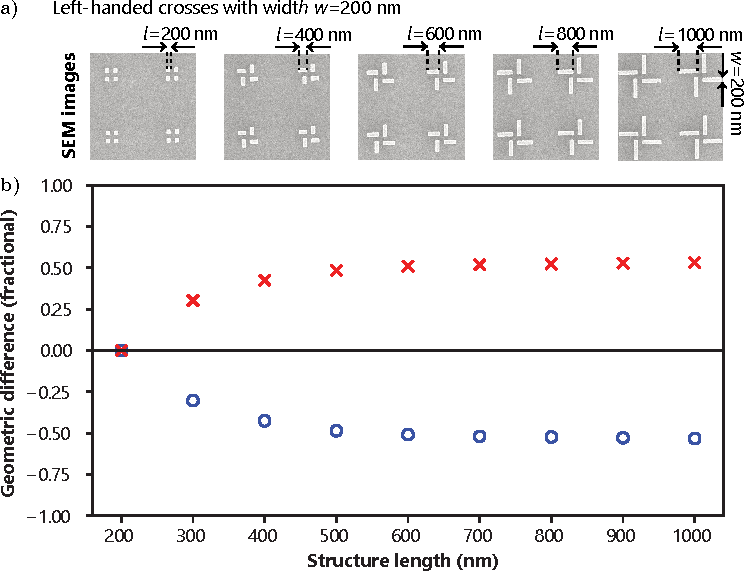
\includegraphics[scale=1]{./figures/results/EnantiomorphingChiralCrosses/d200structures.pdf}
    \caption{\label{fig:results:EnantiomorphingChiralCrosses:d200structures}
    Additional experimental and simulated CID results. Varying arm length of the nanostructure features at fixed $w=\SI{200}{\nano\m}$. \textbf{a)}. SEM images of 4 structure cells for each geometry. \textbf{b)}. Chiral geometric difference for structures of fixed arm width $w=\SI{200}{\nano\m}$.}	
\end{figure}

We further verify this agreement with a second set of intermediate structures (Figure~\ref{fig:results:EnantiomorphingChiralCrosses:d200structures}) in which the nanostripe length is varied, for a constant width of $\SI{200}{\nano\m}$. We observe in both the experiments (originating from near-field) and the near-field simulations that the CID emerges away from the achiral structure, and subsequently plateaus (Figure~\ref{fig:results:EnantiomorphingChiralCrosses:d200data}). Although longer nanostripes support more electromagnetic modes than shorter ones, these additional modes spread across the whole structure, and do not influence dramatically the key central region. The nonlinear CID measurements probe the the center of the crosses and, consiquently, it plateaus as nanostripe length increases.

\begin{figure}[htb!]	
    \centering	
    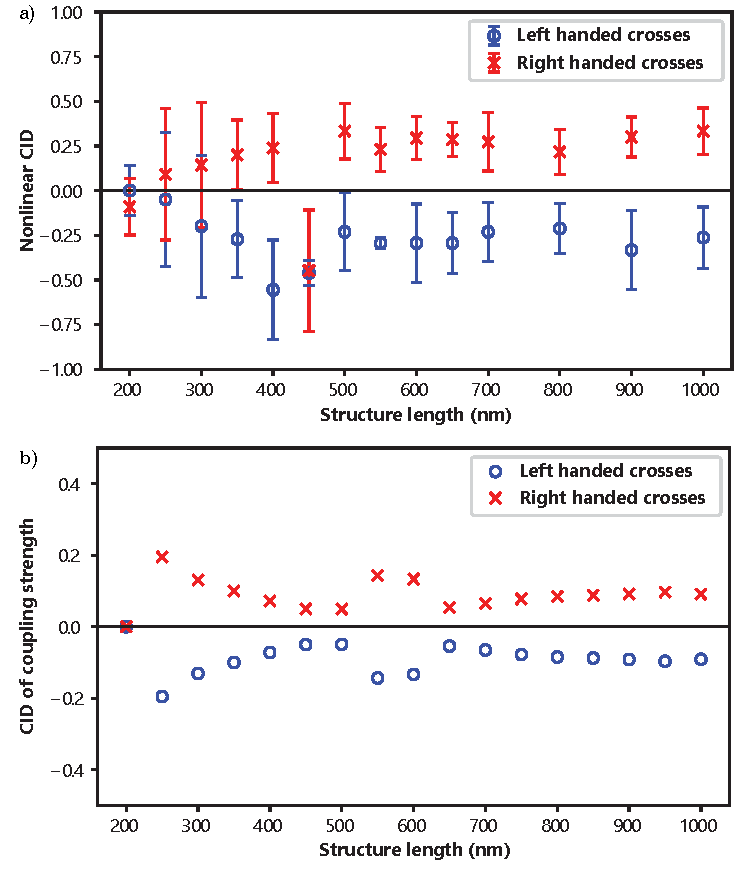
\includegraphics[scale=1]{./figures/results/EnantiomorphingChiralCrosses/d200data.pdf}
    \caption{\label{fig:results:EnantiomorphingChiralCrosses:d200data}
    Additional experimental and simulated CID results. Varying arm length of the nanostructure features at fixed $w=\SI{200}{\nano\m}$. \textbf{a)} Measured total multi-photon CID, and \textbf{(b)} total coupling strength CID obtained from modal analysis, under $w=\SI{800}{\nano\m}$ wavelength light is then calculated for each geometry. Unlike the case of fixed length and varying width, no bisignate CID is observed here, more closely matching the chiral geometric difference.}
\end{figure}

\section{Conclusions}\label{sec:results:EnantiomorphingChiralCrosses:conclusions}

This study has focussed on the bisignate CID response as a function of varying structure geometry. With respect to wavelength, both linear and nonlinear chiroptical spectra often exhibit complex bisignate (of two signs) features~\cite{Li2015, Lee2013, Decker2007, Droulias2013, Plum2009}. This behaviour can be linked to Kuhn’s sum-rule~\cite{Kuhn1930}, which states that the chiroptical response must be zero over all wavelengths. This dependence on wavelength has been analyzed in terms of exciton coupling~\cite{Guerrero-Martinez2011} nanoparticle-nanoparticle Coulomb coupling~\cite{Fan2010}, and energy level hybridization~\cite{Auguie2011a}.
In particular, in the linear optical case it was shown that the energetic ordering of the hybridized modes can be changed, resulting in a reversal of the linear CD, upon making small relative position shifts between L-shaped nanoparticles~\cite{Hentschel2015}.
In the context of our group-theory discussion, the coupling coefficients of each mode pair are highly dependent on the wavelength of light. Changing the wavelength will change which mode pairs are dominant within the set, for a particular structure geometry. In principle, this can also be used to optimize the CID for a fixed structure and variable wavelength. However, it is often desirable, or even necessary, to operate at a particular wavelength, for example if probing molecules attached to the nanostructure surface. In these cases, tuning the structure geometry allows the near-field CID to be optimized around the available wavelength.

To summarize, we have shown that the origin of the chiroptical response in plasmonic nanostructures is due to the selective excitation of available modes, therefore any physical property that affects the modes will allow tuning of the chiroptical response. This mechanism could also be used to explain previous experimental observations of bisignate CID spectra, where different sets of modes can be coupled differently depending on the wavelength of light. Furthermore, we can predict that variation of temperature of the nanostructures (e.g. by laser heating) will change the sets of available modes, due to thermal expansion or a change in permittivity~\cite{Aksyutov1977}, and can lead to tuning the chiroptical response. Further physical processes that involve excitation of specific plasmonic modes (Fano resonance, spasers, electromagnetically induced transparency, etc.) can also be used to tune that response for desired applications (through achieving large chirality parameter). 
In practice, maximizing the chiroptical response in any plasmonic nanostructure is allowed by suppression of the modes that couple to light ``with the wrong chirality''. Equally important, by locally enhancing a particularly strong mode (e.g. via coupling to an auxiliary structure) it is possible to enhance the chiroptical interaction with molecules. In many cases, these molecular interactions will occur at specific wavelength ranges. We show that the chiroptical response at a specific wavelength can be enhanced, and even reversed, by tuning structure geometry alone. This tuneability will lead to improved enantioselectivity for molecular sensing, separation and synthesis.
